\chapter{Development Methodolgy}

\textcolor{red}{\textbf{TODO: Possibly restructure this, it\'s a start for now. Not 100\% sure what Neil\'s looking for here.}}

Upon starting the project, we met as a group and decided on a standard style of development which would work best between all of us. After some discussion, we concluded that a \textit{Scrumban}\cite{scrumban} style of development would best fit our needs. Due to the relatively short duration of the project, and our team consisting of only eight developers, we decided on adopting this rather hands off development approach which focuses on flexibility and being able to change and adapt the project plan and sprints as the project progresses. The \textit{Scrumban} methodology was also suited to the project as the two technologies we were required to use, Java EE and .NET Core, were new to all of the members of our team, making estimating sprints and velocity quite difficult. 

We began the project by breaking the project specification down into disitinct microservices, and deciding which technologies would be best suited to each service. \textbf{TODO: Link to figure below}

\begin{figure}[H]
    \centering
    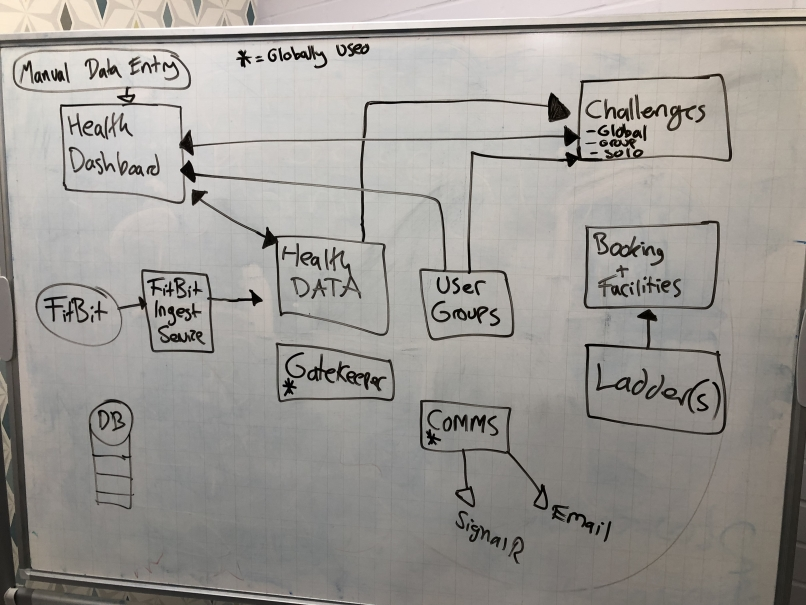
\includegraphics[width=\textwidth]{Images/Initial_Spec_Chart.jpg}
    \caption{An initial design diagram which was used to help break down the project into smaller microservices and gain a rough understanding how each microservice could interact}
\end{figure}

Once the individual microservices had been decided upon, we set out on allocating each microservice to two members of the team and assinging each service a priority ranking between 1 and 3, depending on how the services depended on one another. Services marked with a priority of 1 were core parts of the \textit{AberFitness} infrastructure on which many other parts of the system relied on their APIs in order to function correctly, such as the \textit{Health Data Repository} microservice.  \textbf{TODO: Link to figure below}

\begin{figure}[H]
    \centering
    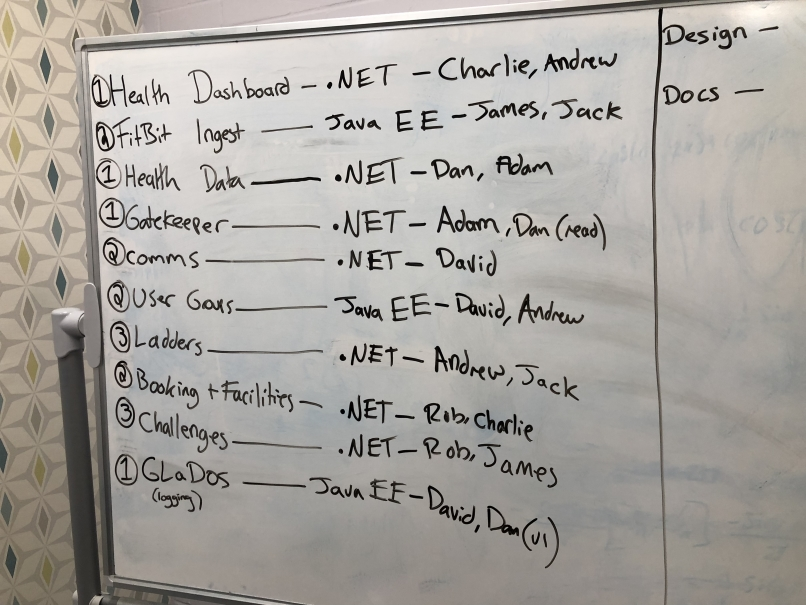
\includegraphics[width=\textwidth]{Images/Numbering_Microservices.jpg}
    \caption{Initial plan for ordering microservices in terms of priority and allocating them to members of the team for development}
\end{figure}